\documentclass[a4paper]{ltjsarticle}

\usepackage[dvipdfmx]{graphicx}
\usepackage[dvipdfmx,hidelinks,pdfusetitle]{hyperref}
\hypersetup{
    colorlinks=false,
    bookmarksnumbered=true,
    pdfborder={0 0 0},
    bookmarkstype=toc
}
\usepackage[nobreak]{cite}
\usepackage{pxjahyper}
\usepackage{amsmath}
\usepackage{tikz}

\usetikzlibrary{datavisualization}
\usetikzlibrary{positioning}
\usetikzlibrary{shapes.geometric, shapes.misc}
\usetikzlibrary{patterns}
\usetikzlibrary{calc}

\begin{document}

% ====================

\begin{itembox}[l]{東京工業大学 2000年 後期}
    実数 $a$,$b$ に対し,$f(x)=x^3+x^2+(a+b-a^2)x+ab$ とおく.

    \begin{enumerate}[label=(\arabic*)]
        \item $f(x)$ を因数分解せよ.

        \item すべての $x\geqq 0$ に対し $f(x)\geqq 0$ が成り立つための $a$,$b$ の条件を求め,それを満たす点 $(a,\ b)$ の存在する範囲を図示せよ.
    \end{enumerate}
\end{itembox}

\begin{enumerate}[label=(\arabic*)]
    \item
          \begin{align*}
              f(x) & =(x+a)b+x\qty(x^2+x+a-a^2) \\
                   & =(x+a)b+x(x+a)(x-a+1)      \\
                   & =(x+a)\qty{b+x(x-a+1)}     \\
                   & =(x+a)\qty{x^2-(a-1)x+b}
          \end{align*}

    \item $g(x)=x^2-(a-1)x+b$ とおくと,

          \begin{equation*}
              g(x)=\qty(x-\frac{a-1}{2})^2+b-\frac{1}{4}(a-1)^2
          \end{equation*}

          $x=0$ のとき,$f(0)=ab\geqq 0$ となる.以下,$x>0$ で考える.

          \begin{enumerate}[label=(\roman*)]
              \item $a\geqq 0$ のとき

                    $x>0$ において $x+a>0$ であるから,$f(x)\geqq 0 \Longleftrightarrow g(x)\geqq 0$

                    よって,軸の位置で分類すると,$a$,$b$ の条件は,

                    \begin{itemize}
                        \item[(ア)] $a\geqq 1$ のとき

                            \begin{equation*}
                                g\qty(\frac{a-1}{2})\geqq 0 \quad \therefore b\geqq \frac{1}{4}(a-1)^2
                            \end{equation*}

                        \item[(イ)] $0\leqq a\leqq 1$ のとき

                            \begin{equation*}
                                g(0)\geqq 0 \quad \therefore b\geqq 0
                            \end{equation*}
                    \end{itemize}

                    となる.

              \item $a<0$ のとき

                    $g(x)$ が $x=-a$ の前後で符号を変えないとすると,$f(x)$ は $x=-a$ の前後で符号が変わるから,$x>0$ において $f(x)\geqq 0$ とはならない.よって, $g(x)$ が $x=-a$ の前後で符号を変えることか必要であり,このとき,

                    \begin{equation*}
                        g(-a)=0 \quad \therefore b=a-2a^2
                    \end{equation*}

                    逆に,$b=a-2a^2$ のとき

                    \begin{align*}
                        g(x)       & =x^2-(a-1)x+a-2a^2=(x+a)(x+1-2a) \\
                        \therefore & f(x)=(x+a)^{2}(x+1-2a)
                    \end{align*}

                    となるから,$a<0$ より,$x\geqq 0$ において $f(x)\geqq 0$ となり十分である.
          \end{enumerate}

          以上から,$(a,\ b)$ の存在範囲は図の網目部分及び太線部分となる.ただし,境界を含む.

          \begin{figure}[!ht]
              \centering
              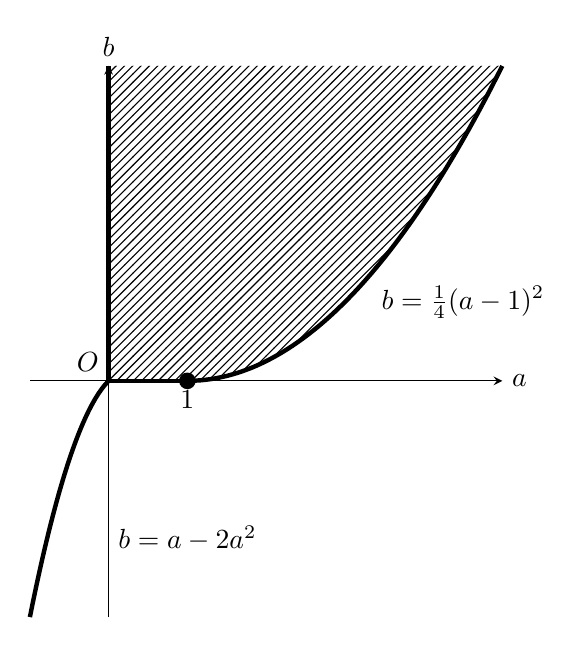
\begin{tikzpicture}
                  \draw[domain=1:5, smooth, variable=\x, ultra thick] plot ({\x},{0.25*(\x-1)^2}) node at (4.5,1) {$b=\frac{1}{4}(a-1)^2$};
                  \fill[gray!80, pattern=north east lines] (0,0) -- plot[domain=1:5] (\x, {0.25*(\x-1)^2}) -- (0,4) -- cycle;
                  \draw[ultra thick] (0,0) -- (1,0);
                  \draw[ultra thick] (0,0) -- (0,4);
                  \draw[domain=-1:0, smooth, variable=\x, ultra thick] plot (\x, {\x-2*\x*\x}) node at (1, -2) {$b=a-2a^2$};
                  \node[below] at (1, 0) {$1$};
                  \fill (1,0) circle (3pt);

                  \draw[->,>=stealth] (-1,0) -- (5,0) node[right] {$a$};
                  \draw[->,>=stealth] (0,-3) -- (0,4) node[above] {$b$};
                  \node[above left] at (0,0) {$O$};
              \end{tikzpicture}
          \end{figure}
\end{enumerate}

% ====================

\end{document}
